\documentclass[12pt]{article}
\usepackage[margin=1in]{geometry}
\usepackage{graphicx}
\usepackage{caption}
\usepackage{booktabs}
\usepackage{float}
\usepackage{pdflscape}
\usepackage{longtable}
\usepackage{hyperref}
\usepackage{inputenc}

\title{Jakarta Indoor PM$_{2.5}$ --- All Figures and Tables}
\date{\today}

\begin{document}
\maketitle
\tableofcontents
\newpage

% =====================================================================
\section{Main Figures}
% =====================================================================

\begin{figure}[H]
  \centering
  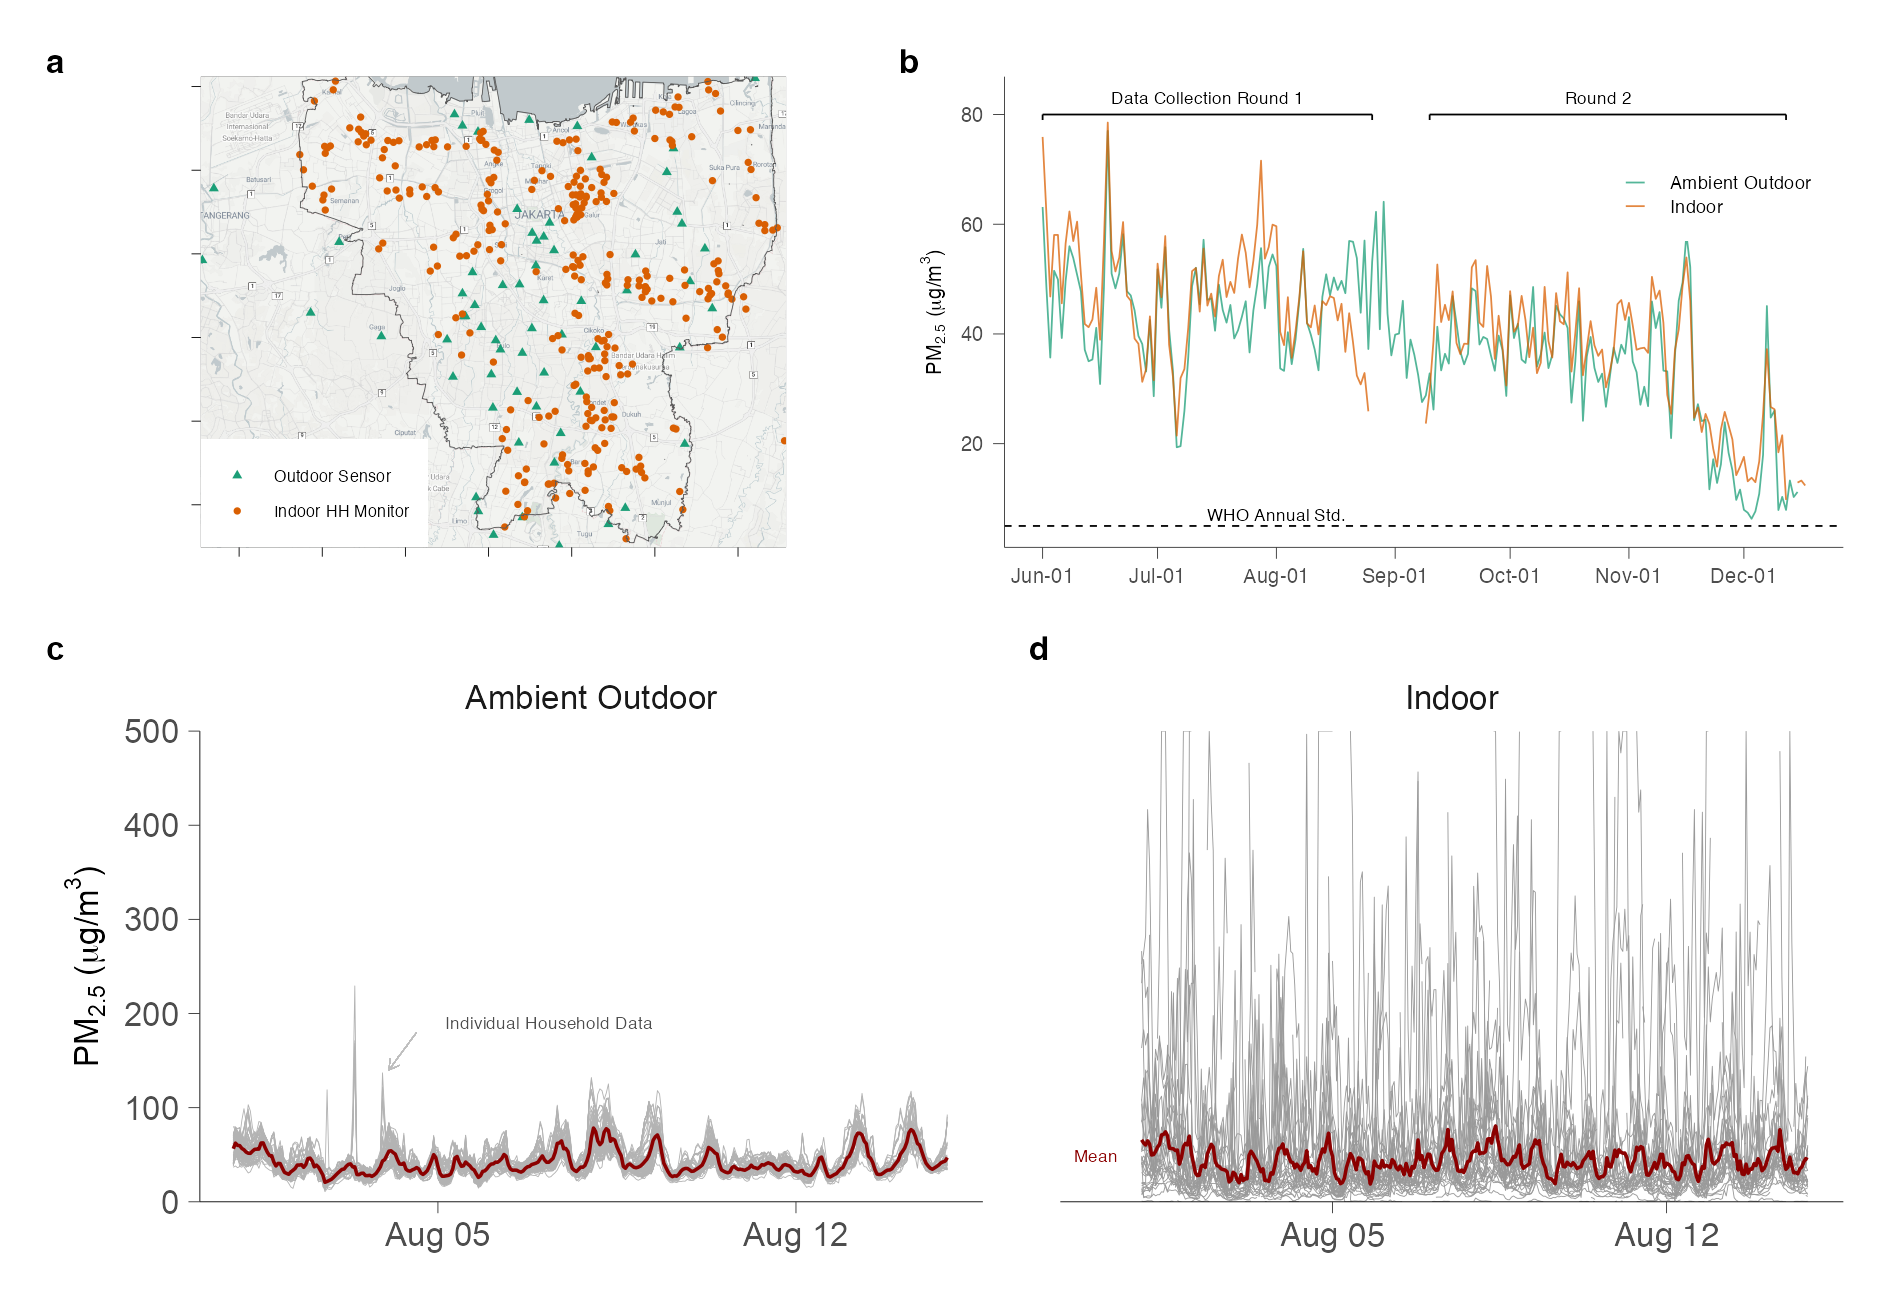
\includegraphics[width=\textwidth]{figures/fig1_desc.png}
  \caption{\textbf{Figure 1: Indoor and Outdoor PM$_{2.5}$ in Jakarta.}
  (a) Locations of respondents and installed air quality monitoring hardware.
  (b) Daily average outdoor and indoor pollution levels.
  (c) Hourly outdoor PM$_{2.5}$ Aug 1--14, 2024.
  (d) Hourly indoor PM$_{2.5}$ Aug 1--14, 2024.}
  \label{fig:fig1}
\end{figure}

\newpage
\begin{figure}[H]
  \centering
  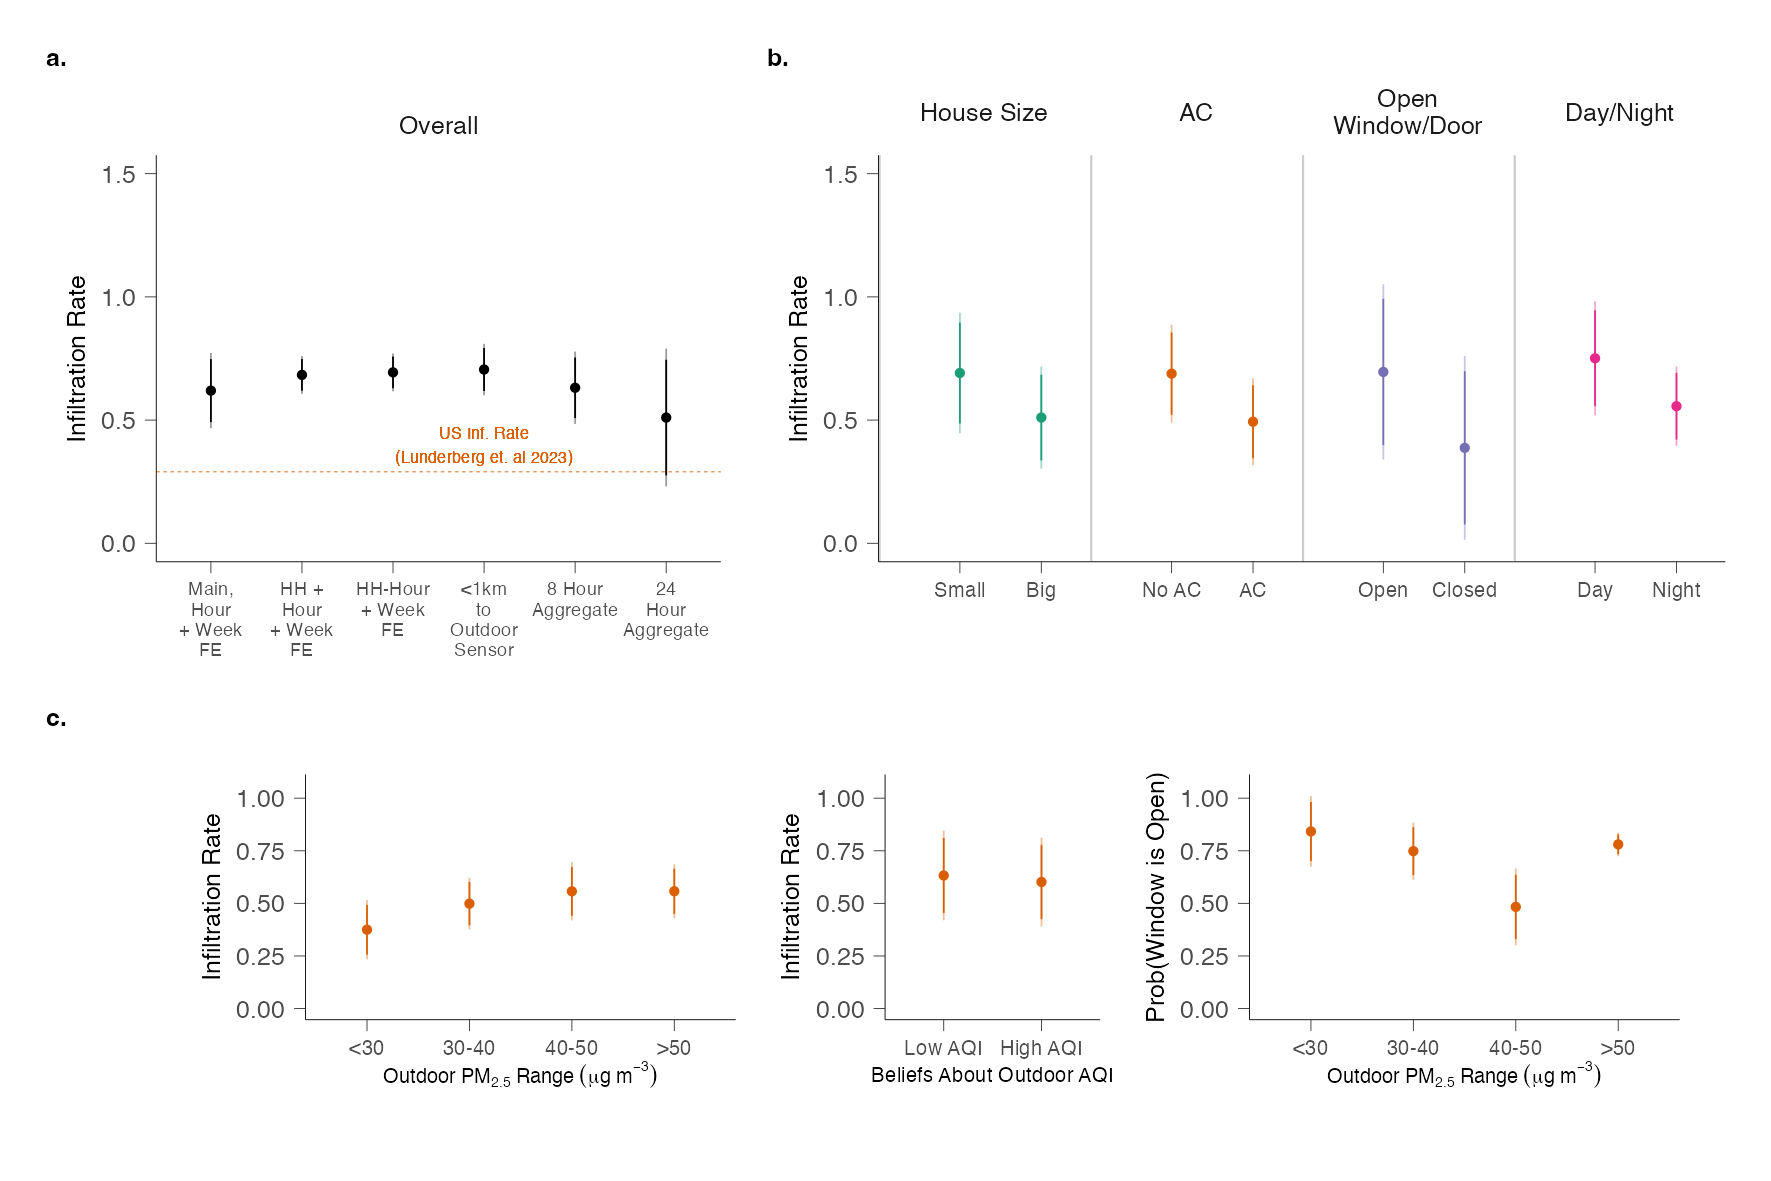
\includegraphics[width=\textwidth]{figures/fig2_infiltation.png}
  \caption{\textbf{Figure 2: Infiltration Rate from Ambient Outdoor to Indoor Homes.}
  (a) Infiltration rates across regression specifications, including the new 24-hour aggregate model.
  Specifications: (1) Main rhs\_fml controls + hour/week FE; (2) HH + Hour + Week FE;
  (3) HH-Hour + Week FE; (4) $<$1km to outdoor sensor; (5) 24-hour aggregate, week FE.
  All regressions upweight hours with higher rates of missing indoor PM$_{2.5}$.
  (b) Heterogeneity in infiltration rates by household characteristics (income moved to Figure 4).
  (c) Household behavioral responses to outdoor pollution levels.}
  \label{fig:fig2}
\end{figure}

\newpage
\begin{figure}[H]
  \centering
  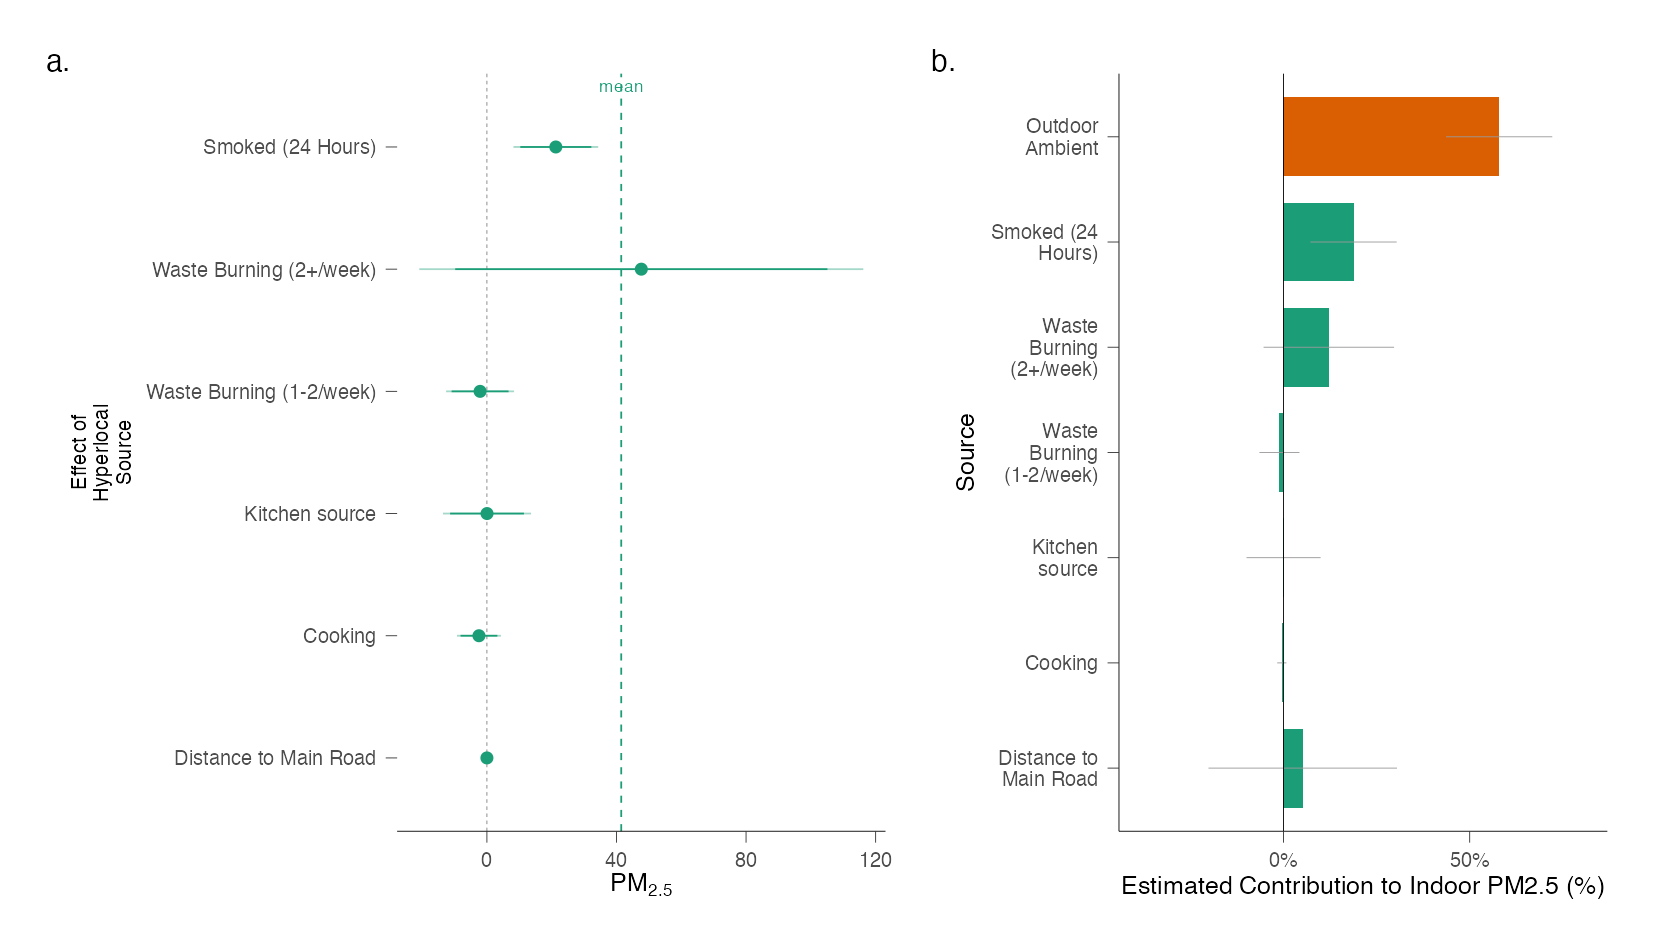
\includegraphics[width=\textwidth]{figures/fig3_sources.png}
  \caption{\textbf{Figure 3: Contributions of Hyperlocal Pollution.}
  (a) Regression coefficients of indoor PM$_{2.5}$ on indoor pollution-generating activities:
  smoking (24 hours), waste burning (1-2/week and $>$2/week), kitchen/cooking proximity,
  cooking indicator, and distance to main road.
  Dashed line shows sample mean indoor PM$_{2.5}$.
  (b) Mean contribution decomposition: fraction of mean indoor PM$_{2.5}$ attributed to
  ambient outdoor infiltration versus hyperlocal sources.}
  \label{fig:fig3}
\end{figure}

\newpage
\begin{figure}[H]
  \centering
  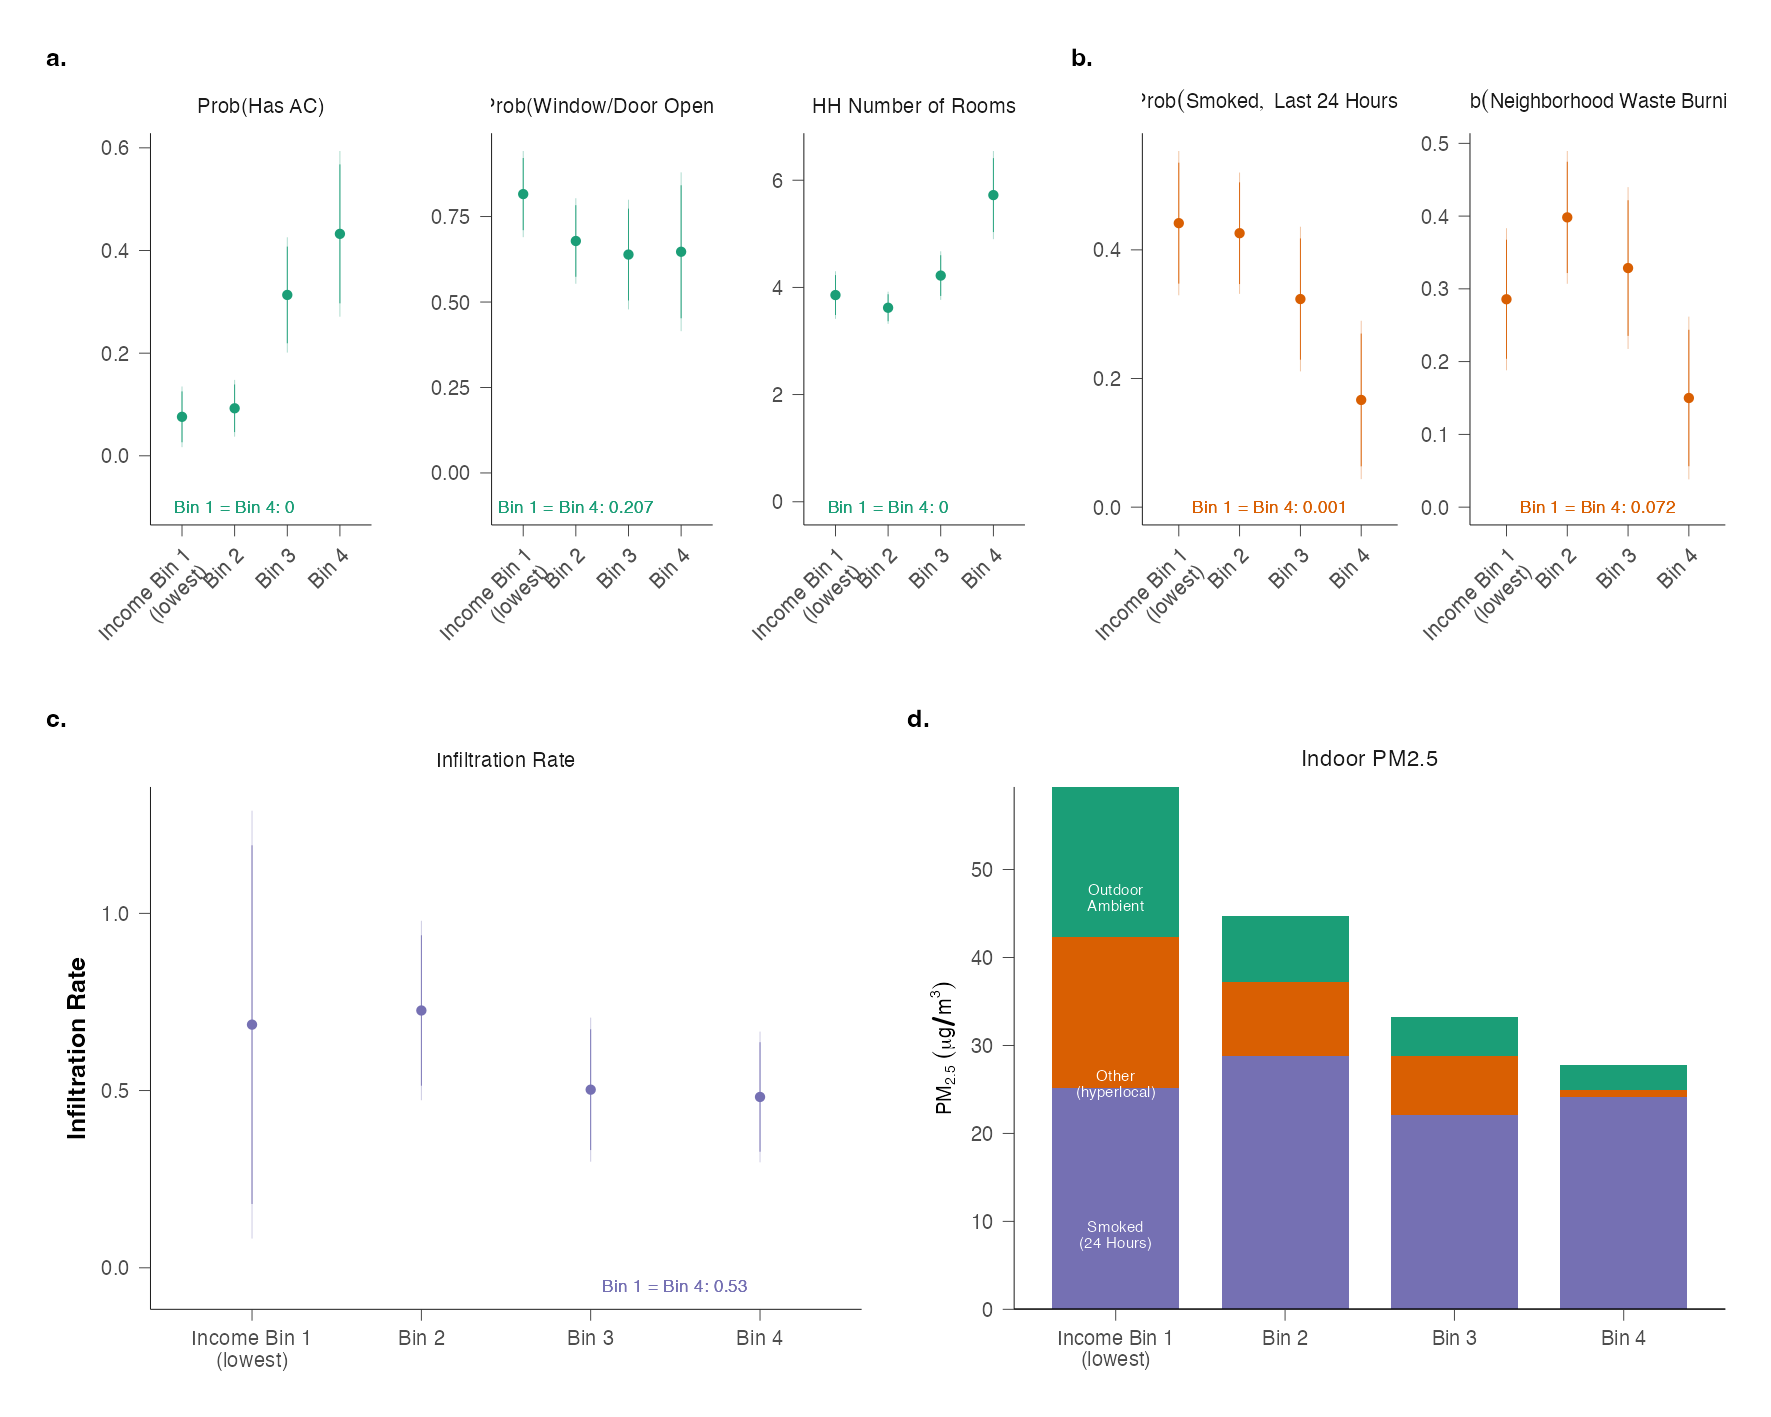
\includegraphics[width=\textwidth]{figures/fig4_pm_income.png}
  \caption{\textbf{Figure 4: Indoor PM$_{2.5}$ Higher for Lower Income Households.}
  (a) Household characteristics by income quartile (AC ownership, window/door open,
  number of rooms).
  (b) Hyperlocal pollution sources by income quartile (neighborhood waste burning,
  indoor smoking).
  (c) Infiltration rate heterogeneity by income quartile (moved from Figure 2).
  (d) Decomposition of indoor PM$_{2.5}$ by income quartile into ambient outdoor,
  smoking, and other (hyperlocal) contributions.}
  \label{fig:fig4}
\end{figure}


% =====================================================================
\section{Appendix Figures}
% =====================================================================

\begin{figure}[H]
  \centering
  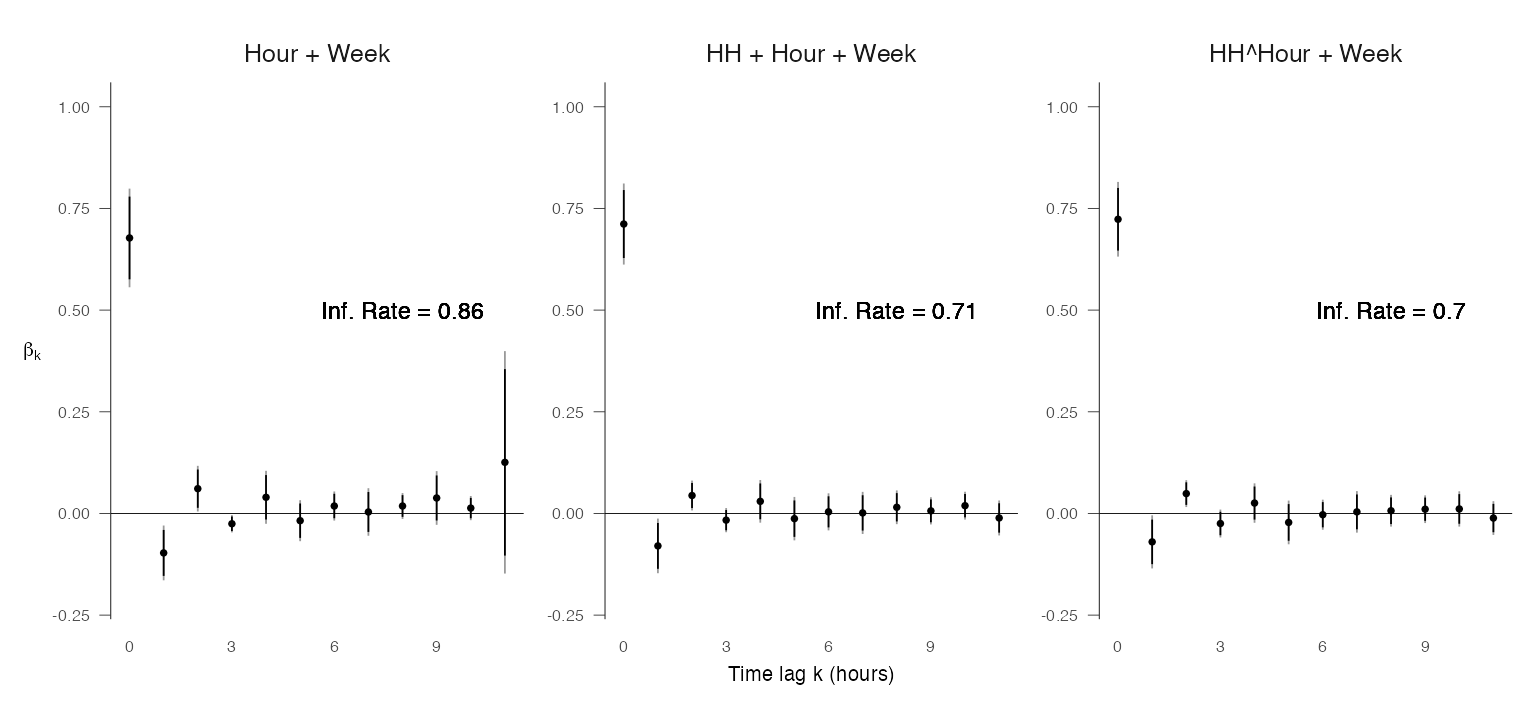
\includegraphics[width=\textwidth]{figures/inf_lags.png}
  \caption{\textbf{Figure A1: Infiltration Rate with Lagged Outdoor PM$_{2.5}$.}
  Distributed-lag specification showing infiltration $\beta_k$ coefficients for lags $k = 0, \ldots, 11$ hours,
  across three fixed-effect specifications. The cumulative infiltration rate (sum of $\beta_k$) is annotated.}
  \label{fig:A1}
\end{figure}

\newpage
\begin{figure}[H]
  \centering
  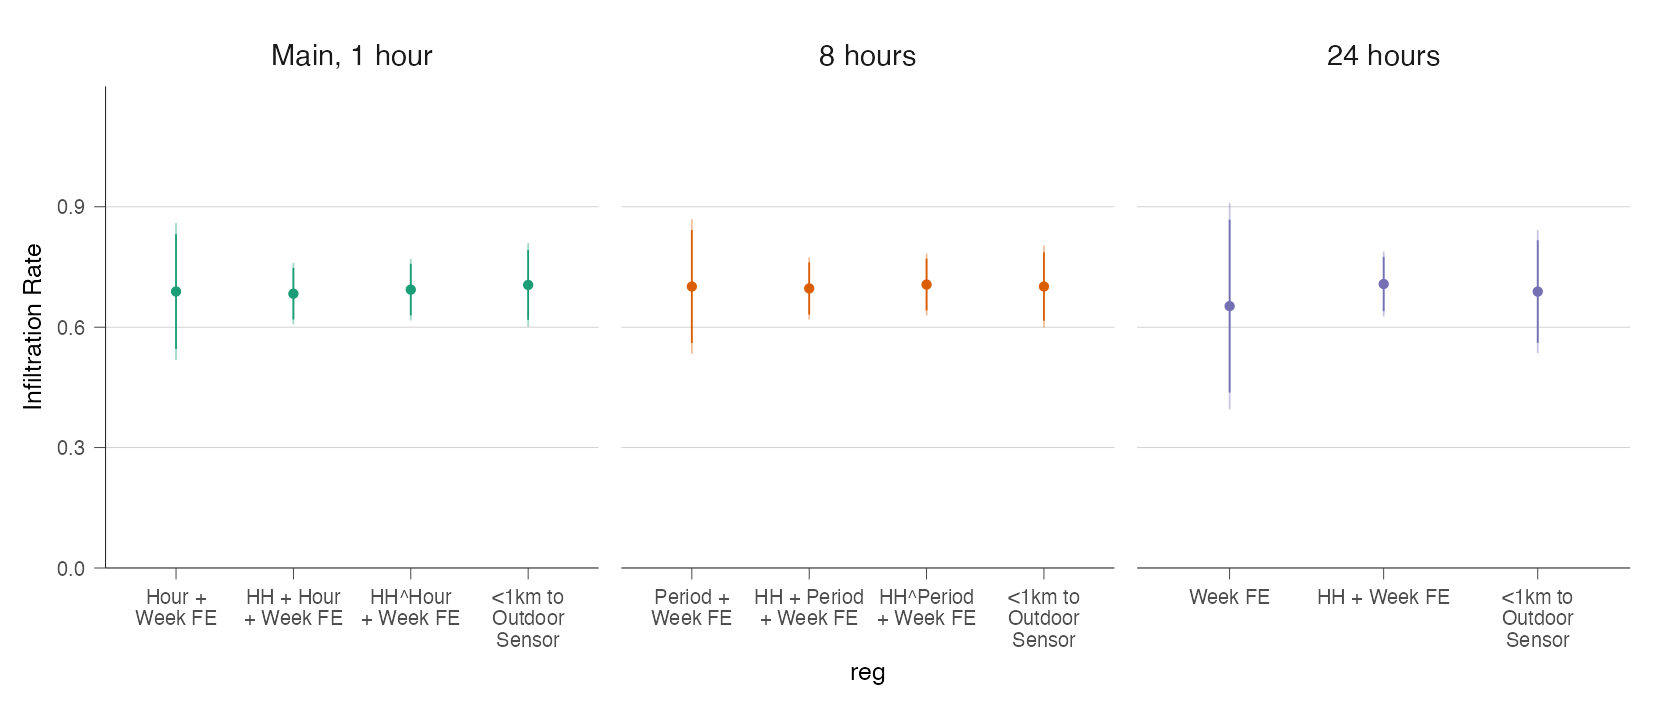
\includegraphics[width=\textwidth]{figures/inf_aggregation.png}
  \caption{\textbf{Figure A2: Infiltration Rate at Different Aggregation Levels.}
  Infiltration rates estimated at 1-hour, 8-hour, and 24-hour averaging periods, across multiple
  fixed-effect specifications. Results are consistent across temporal resolutions.}
  \label{fig:A2}
\end{figure}

\newpage
\begin{figure}[H]
  \centering
  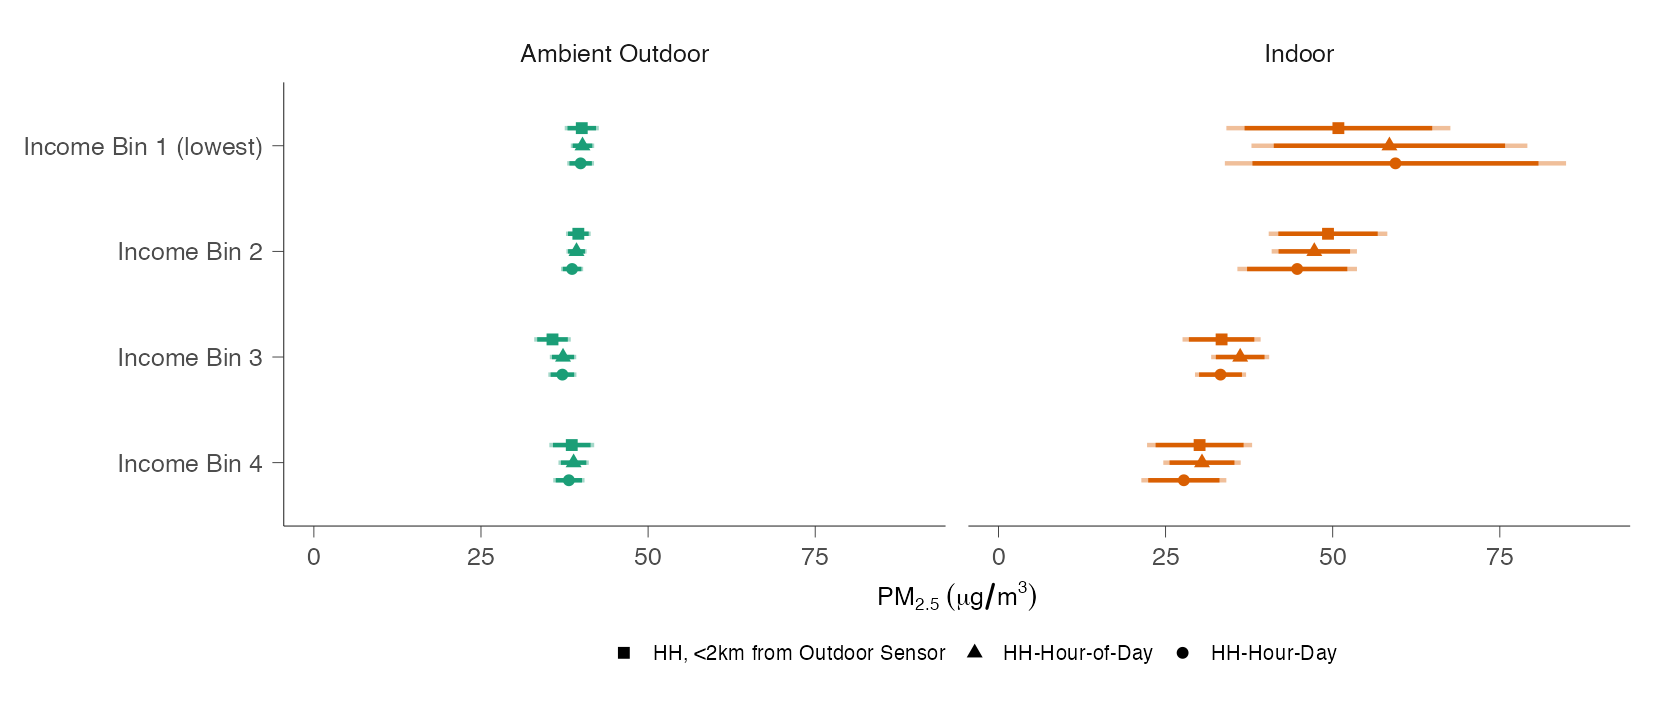
\includegraphics[width=\textwidth]{figures/pm_income_robustness.png}
  \caption{\textbf{Figure A3: Robustness --- Mean PM$_{2.5}$ Under Various Aggregation Methods.}
  Mean PM$_{2.5}$ concentrations by income quartile using three aggregation approaches:
  household-level with $<$2km sensor proximity, household-hour-of-day averages,
  and household-hour-date averages.}
  \label{fig:A3}
\end{figure}

\newpage
\begin{figure}[H]
  \centering
  \IfFileExists{figures/fig_appendix_spike_sources.png}{%
    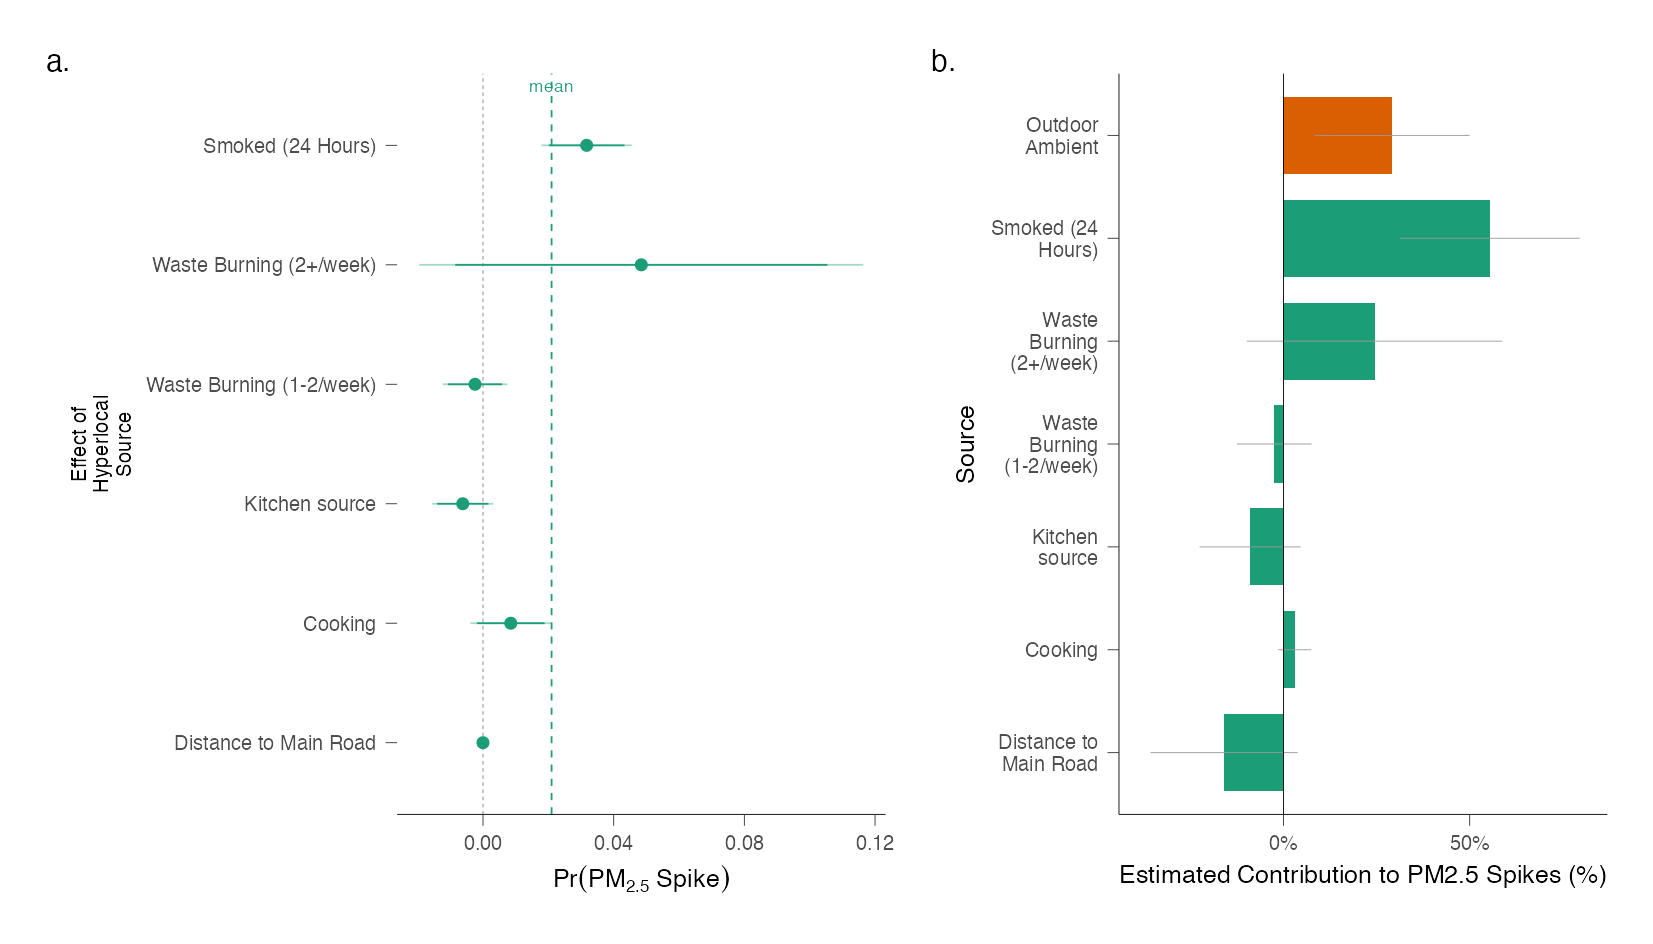
\includegraphics[width=0.75\textwidth]{figures/fig_appendix_spike_sources.png}%
  }{%
    \fbox{\parbox{0.75\textwidth}{\centering\vspace{2cm}
      \textit{[Figure A4 not yet generated. Run updated appendix.R to produce\\
      \texttt{output/figures/fig\_appendix\_spike\_sources.png}]}\vspace{2cm}}}%
  }
  \caption{\textbf{Figure A4: Source Contributions to PM$_{2.5}$ Spikes.}
  Mean contribution decomposition with PM$_{2.5}$ spikes ($>125.5~\mu$g/m$^3$, the EPA ``Very Unhealthy''
  threshold) as the outcome. Fraction of mean spike probability attributed to each source.
  Note: this figure is generated after running the updated code.}
  \label{fig:A4}
\end{figure}

\newpage
\begin{figure}[H]
  \centering
  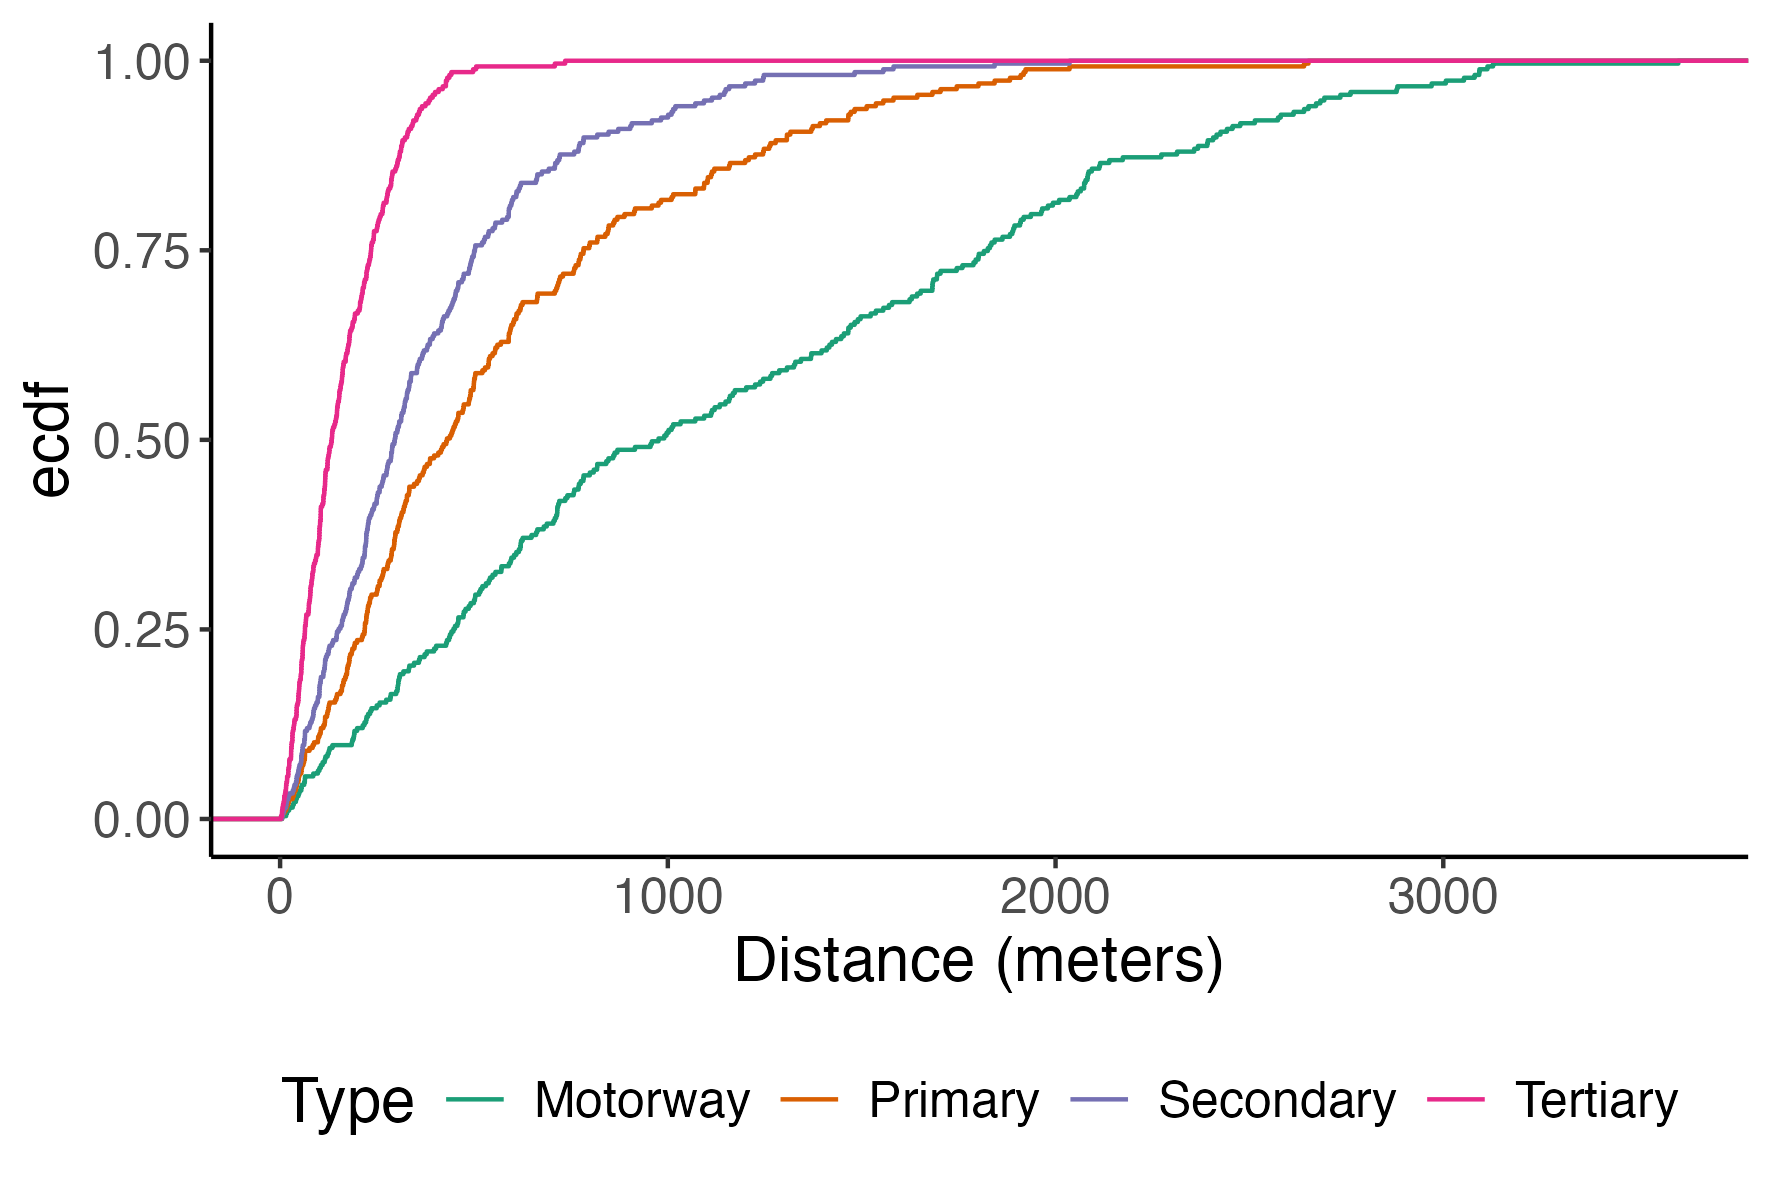
\includegraphics[width=0.75\textwidth]{figures/distance_to_road_ecdf.png}
  \caption{\textbf{Figure A5: ECDF of Distance to Roads.}
  Empirical cumulative distribution of household distance to motorway, primary,
  secondary, and tertiary roads.}
  \label{fig:A5}
\end{figure}

\newpage
\begin{landscape}
\begin{figure}[H]
  \centering
  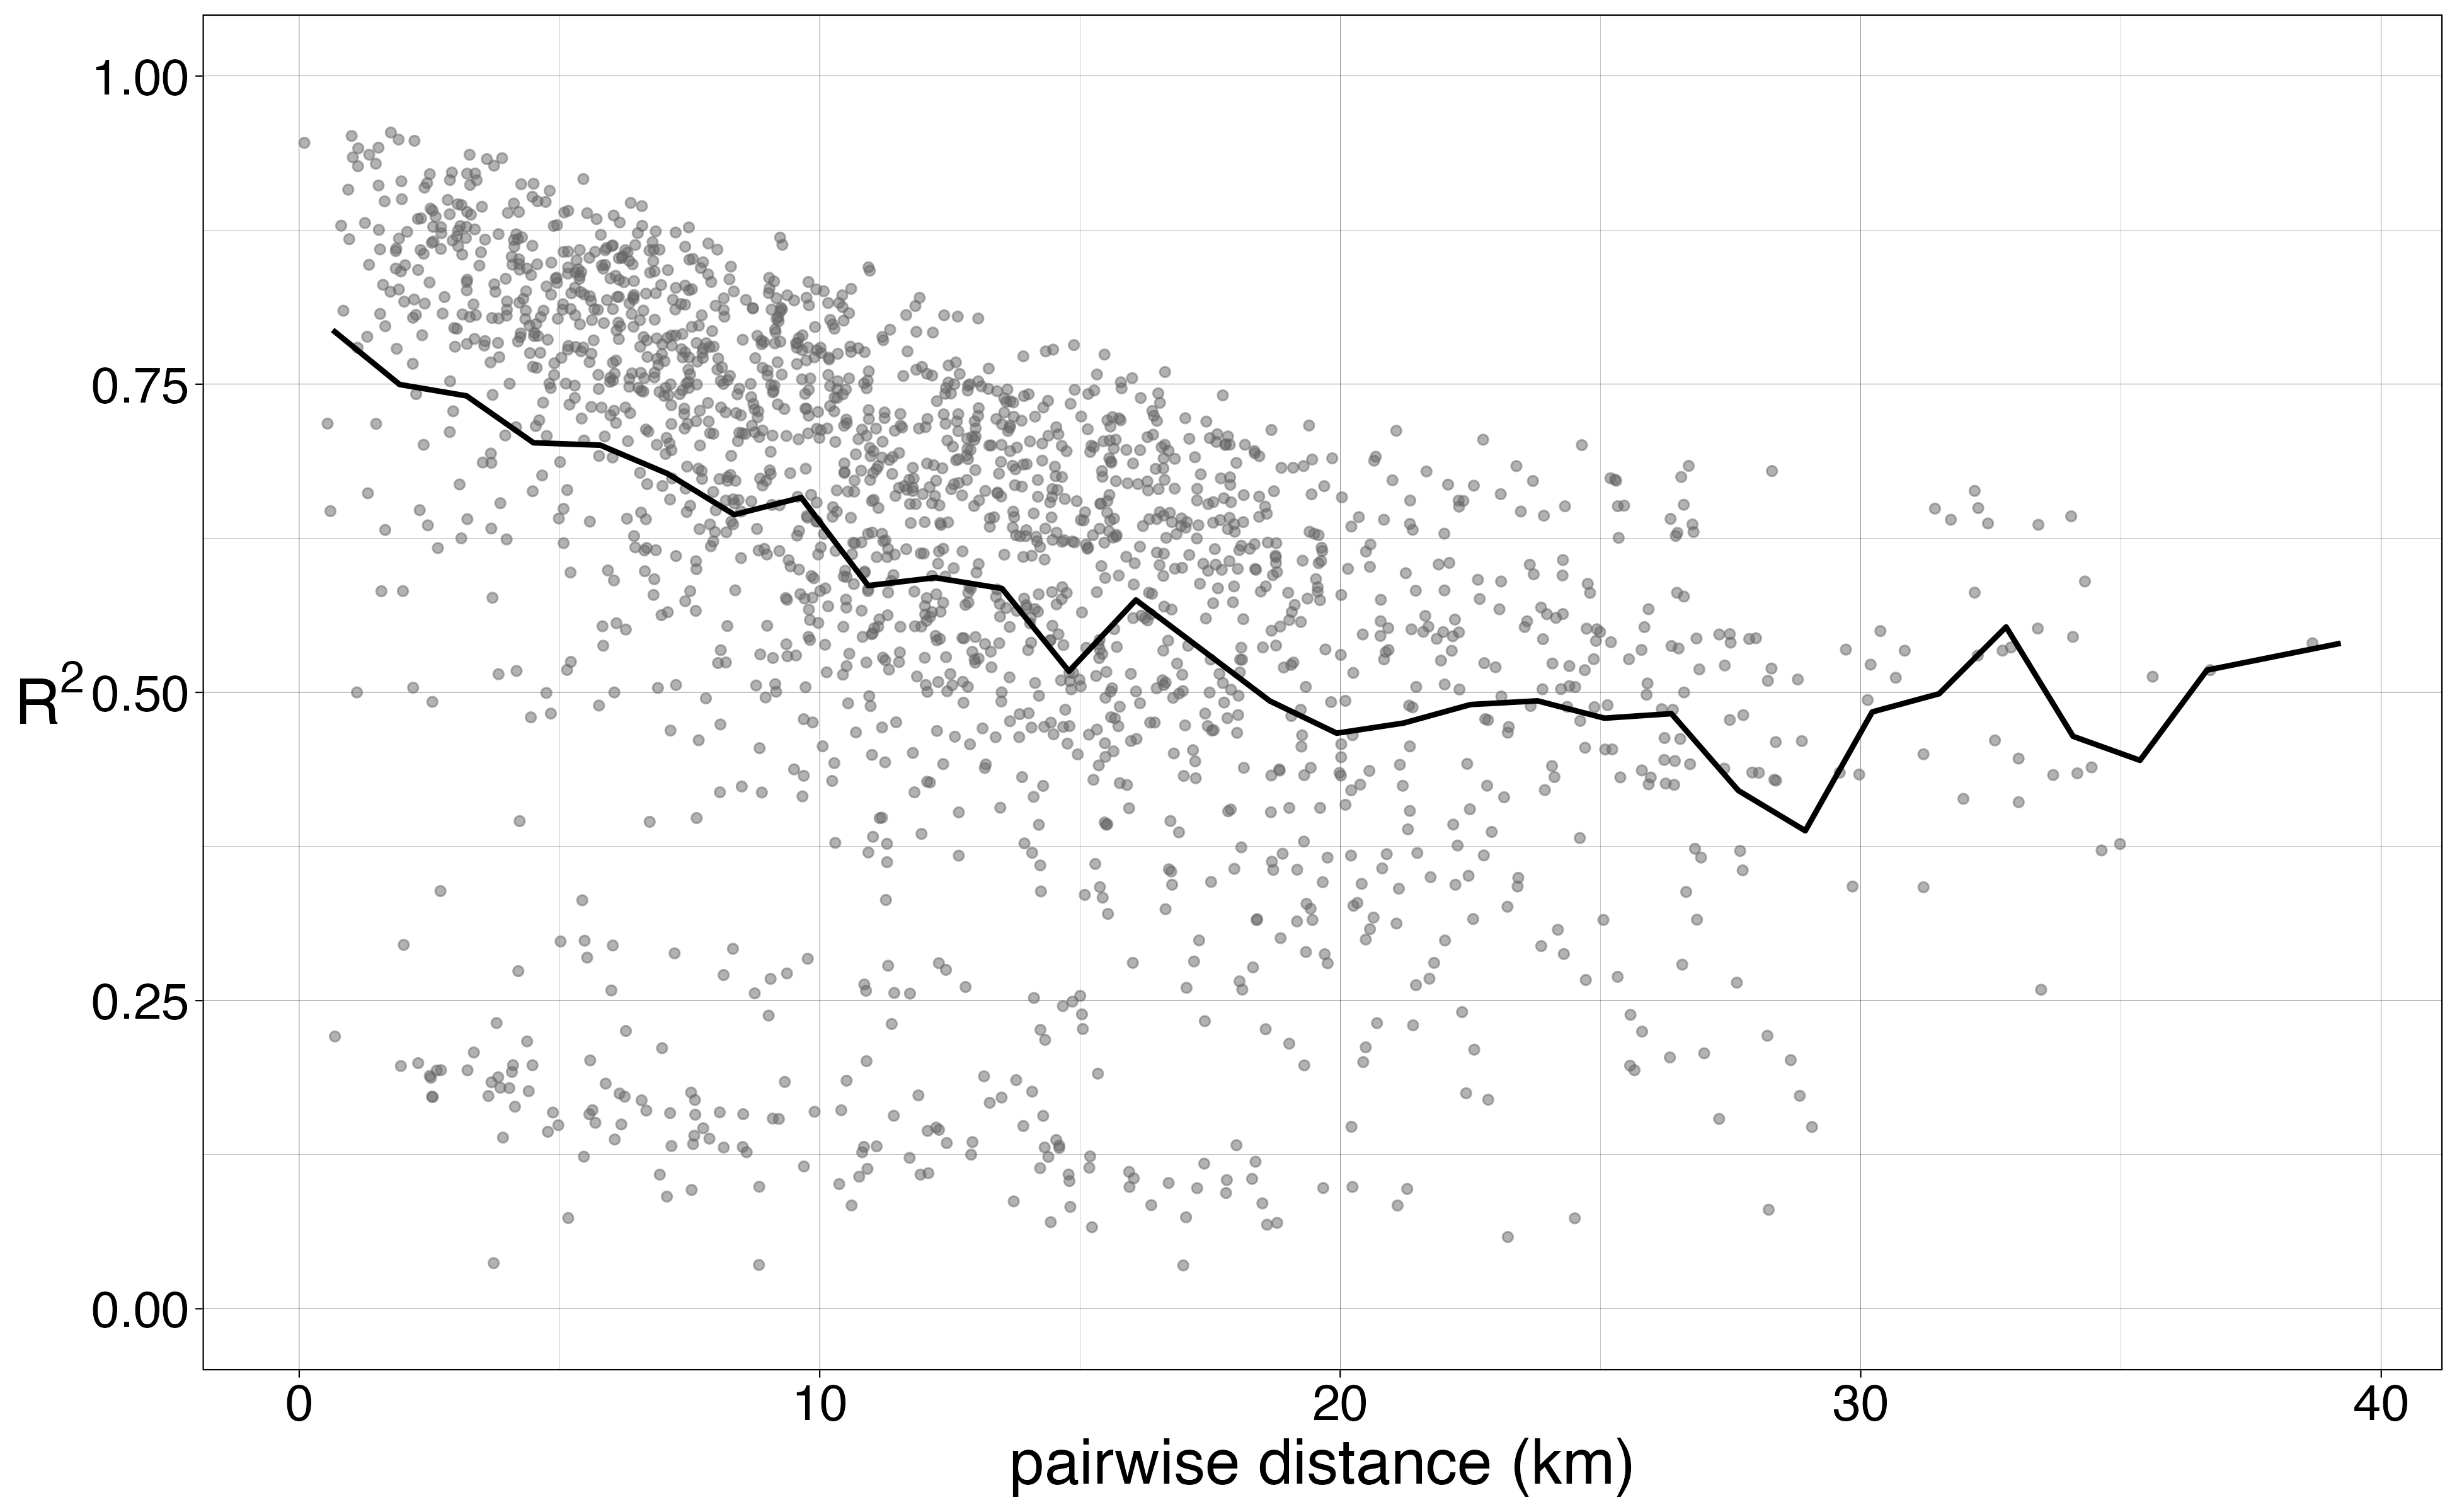
\includegraphics[width=0.9\linewidth]{figures/sensor_correlations.png}
  \caption{\textbf{Figure A6: Spatial Correlation between Outdoor Sensors.}
  Pairwise $R^2$ of log-PM$_{2.5}$ between sensor pairs as a function of distance.
  Outdoor pollution is highly spatially correlated even at distances $>$10 km.}
  \label{fig:A6}
\end{figure}
\end{landscape}


% =====================================================================
\section{Main Tables}
% =====================================================================


\begin{tabular}{cccccc}
\toprule
Source & Reg. Estimate & p.value & Mean Value of Source & Mean Contribution & $R^2$ Contribution\\
\midrule
Outdoor Ambient & 0.59 & 0.000 & 39.41 & 56\% & 33\%\\
Smoked (24 Hours) & 21.33 & 0.001 & 0.38 & 19\% & 23\%\\
Kitchen source & -0.28 & 0.968 & 0.31 & 0\% & 0\%\\
Cooking & -2.49 & 0.469 & 0.08 & 0\% & 0\%\\
Distance to Main Road (km) & 3.52 & 0.707 & 0.57 & 5\% & 0\%\\
\addlinespace
Waste Burning (1-2/week) & -1.76 & 0.743 & 0.21 & -1\% & \\
Waste Burning (3+/week) & 46.85 & 0.168 & 0.10 & 12\% & \\
 &  &  &  &  & 22\%\\
\bottomrule
\end{tabular}


% =====================================================================
\section{Appendix Tables}
% =====================================================================

\begin{table}[H]
  \centering
  \caption{\textbf{Table A1: Summary Statistics of Household Survey.}
  Household characteristics from the study sample compared to the Jakarta population mean
  from SUSENAS 2023.}
  
\begin{tabular}{lccc}
\toprule
Variable & Control Mean & N & Population Mean\\
\midrule
Female & 0.9 & 283 & \\
 &  &  \vphantom{3} & \\
Age & 41.21 & 283 & \\
 & (6.91) &  & \\
HH Size & 5.13 & 283 & 3.79\\
 & (1.94) &  & (1.31)\\
Number of Children & 2.05 & 283 & \\
 & (1.03) &  & \\
HH Monthly Exp. (USD) & 248.74 & 275 & 655.94\\
 & (117.16) &  & (707.71)\\
HH Monthly Income (USD) & 312.48 & 281 & \\
 & (194.17) &  & \\
HH Head Attended Secondary & 0.88 & 283 & 0.88\\
 &  &  \vphantom{2} & \\
HH Head Attended Tertiary & 0.14 & 283 & 0.3\\
 &  &  \vphantom{1} & \\
Owns AC & 0.55 & 282 & 0.39\\
 & (0.5) &  & \\
LPG Stove & 0.98 & 283 & 0.96\\
 &  &  & \\
Number of Smokers & 0.93 & 283 & 0.73\\
 & (0.85) &  & (0.71)\\
\midrule
\bottomrule
\end{tabular}

  \label{tab:covariates}
\end{table}

\newpage
\begin{table}[H]
  \centering
  \caption{\textbf{Table A2: Distance to Outdoor Sensor Not Correlated with Household Characteristics.}
  Regression of household distance to nearest outdoor sensor on household covariates.
  No evidence of selection bias on observables.}
  
\begin{tabular}{lc}
   \toprule
   Dependent Variable:           & Distance to Outdoor Sensor (meters)\\  
   Model:                        & (1)\\  
   \midrule
   \emph{Variables}\\
   Indoor PM2.5                  & -0.99\\   
                                 & (2.44)\\   
   Outdoor PM2.5                 & 1.19\\   
                                 & (9.21)\\   
   Income (USD)                  & 0.13\\   
                                 & (0.58)\\   
   Housing Size                  & 42.52\\   
                                 & (53.36)\\   
   AC                            & -198.33\\   
                                 & (197.47)\\   
   HOH Employed                  & 314.69\\   
                                 & (374.62)\\   
   HOH Attended Secondary School & -285.71\\   
                                 & (305.55)\\   
   HOH Attended Tertiary School  & -173.15\\   
                                 & (317.86)\\   
   \midrule
   \emph{Fit statistics}\\
   Dependent variable mean       & 2,337.6\\  
   Observations                  & 283\\  
   \bottomrule
\end{tabular}



  \label{tab:sensor_selection}
\end{table}

\newpage
\begin{table}[H]
  \centering
  \caption{\textbf{Table A3: Waste Burning Not Correlated with Higher Ambient Outdoor PM$_{2.5}$.}
  Regression of outdoor PM$_{2.5}$ on reported neighborhood waste burning frequency,
  for all households and restricting to households within 2km of a sensor.}
  
\begingroup
\centering
\begin{tabular}{lcc}
   \tabularnewline \midrule \midrule
   Dependent Variable: & \multicolumn{2}{c}{Outdoor PM2.5}\\
                            & Closest 3 Sensors & HH Within 2km of Outdoor Sensor \\   
   Model:                   & (1)               & (2)\\  
   \midrule
   \emph{Variables}\\
   Waste Burning (1-2/week) & 0.900             & 0.410\\   
                            & (0.770)           & (0.734)\\   
   Waste Burning (3+/week)  & 3.65$^{***}$      & 5.25$^{***}$\\   
                            & (0.991)           & (1.79)\\   
   Outdoor Temperature      & -0.380            & 0.145\\   
                            & (0.243)           & (0.255)\\   
   Outdoor Humidity         & -0.194$^{***}$    & -0.180$^{***}$\\   
                            & (0.042)           & (0.048)\\   
   \midrule
   \emph{Fixed-effects}\\
   Week FE                  & Yes               & Yes\\  
   Hour FE                  & Yes               & Yes\\  
   \midrule
   \emph{Fit statistics}\\
   Observations             & 823,850           & 423,609\\  
   R$^2$                    & 0.38558           & 0.37695\\  
   Within R$^2$             & 0.00940           & 0.01310\\  
   \midrule \midrule
   \multicolumn{3}{l}{\emph{Clustered (respondent\_id \& date\_hour) standard-errors in parentheses}}\\
   \multicolumn{3}{l}{\emph{Signif. Codes: ***: 0.01, **: 0.05, *: 0.1}}\\
\end{tabular}
\par\endgroup



  \label{tab:outdoor_burning}
\end{table}

\newpage

\begin{tabular}{cccccc}
\toprule
Source & Reg. Estimate & p.value & Mean Value of Source & Mean Contribution & $R^2$ Contribution\\
\midrule
Outdoor Ambient & 0.000 & 0.008 & 39.41 & 28\% & 2\%\\
Smoking Household & 0.032 & 0.000 & 0.38 & 57\% & 54\%\\
Kitchen source & -0.006 & 0.180 & 0.31 & -9\% & 2\%\\
Cooking & 0.008 & 0.191 & 0.08 & 3\% & 1\%\\
Distance to Main Road (km) & -0.006 & 0.109 & 0.57 & -16\% & 5\%\\
\addlinespace
Waste Burning (1-2/week) & -0.002 & 0.663 & 0.21 & -2\% & \\
Waste Burning (3+/week) & 0.047 & 0.164 & 0.10 & 23\% & \\
 &  &  &  &  & 19\%\\
\bottomrule
\end{tabular}


\end{document}
